\documentclass[letterpaper, 10pt]{article}

\usepackage[letterpaper, margin=1in]{geometry}
\usepackage{indentfirst}
\usepackage{multicol}
\usepackage{graphicx}
\graphicspath{ {./} }

\begin{document}

\title{Attention Mechanisms for Recurrent Neural Networks}
\author{Roland Laboulaye and Brandon Schoenfeld}
\date{April 12, 2018}
\maketitle

\begin{multicols}{2}

\noindent \textbf{Abstract.}
We explore the use of a recurrent neural network (RNN) with a gated recurrent unit (GRU) to solve
the task of neural mchine translation (NMT). Futhermore, we apply an attention mechanism to allow
the RNN to learn which words of the input sentence are important at each step of translation.

\section{Introduction}
Given a corpus of written sentences in one language with corresponding sentence translations in
another language, we would like to train a deep neural network to learn a model which maps from the
original language to the translated, which having generalizing capabilities to translate novel
sentences.
Translation is difficult for humans, even after years of study and practice, and is often best
performed by those who have studied and used the two languages in question from their nativity.
Any technology which can quickly and reliably complete this task is highly desirable and can be used
in many applications.

One common approach to neural machine translation (NMT) uses a recurrent neural network (RNN) with
a gated recurrent unit (GRU).
The RNN model is capable of learning patterns in time-series data,
like sentences, with variable length.
The GRU is an internal component to the RNN which allows the model to persist a memory state between
time steps, or words, in the sentence.
We apply an attention mechanism, proposed by Bahdanau, et. al. \textsuperscript{[1]}, which further
enhances the translation process by allowing the RNN to observe data from every time step in the
sequence, not just the previous.

% Automatic text-to-text translation presents several challenges for any machine learning algorithm.
% While some machine learning tasks have data with instances of a fized size, sentences come in many
% different sizes; it can be terse or overly verbose.
% Additionally, this problem is compounded as the target translation language has the same problem.
% The algorithm must be able to map from any length of sentence to any length of translated sentence.
% In one language, there can be many ways to express the same general meaning.
% With two languages, there is a many-to-many problem where any one form of a sentence could be
% legitimately translated into any one of the valid target sentence forms.
% Thirdly, both languages typically have a large vocabulary with hundreds of thousands of words.
% Each word has to be encoded using some mechanism to allow the computer to analyze it.
% With a large vocabularly, a high dimensional encoding is necessary to uniquely and unambigously
% represent all the words in a language.
% If a language has 100,000 words, a vector of size 100,000 filled with all zeros except a single one,
% indicating
% One alternative is a lower, but still high dimensional, learned embedding, like FastText[citation needed]
% which 
% encoding/embedding

\section{Background}
\subsection{RNN Encoder-Decoder}

In typical neural machine translation, an encoder-decoder structure is used.
In such approaches, the encoder, an RNN, produces a hidden state for each token in the input
sequence.
At each time step in the sequence, the hidden state is a function of the input token and the hidden
state of the previous input token.
Then the decoder, another RNN, uses the state vector from the encoder as its initial state to
generate new words, updating the its state with each new word generation.
One chief weakness of this approach is that the way that the hidden states from the original
encoding are compressed might not be optimal for each distinct step of the decoding process.
In fact, in many implementations, only the final hidden state of the encoder is preserved as the
encoding of the entire input.
This dramatically limits the length of sequences that can be translated, since in long sentences,
signal from early input words might be slowly diluted.

\subsection{GRU}

At each time step of an RNN, there must be some function to combine any state rom the last time
step and the input at the current time step.
One solution is the gated recurrent unit (GRU)\textsuperscript{[2]}.
A GRU takes two inputs, the input data at time $t$ and the ouput of the GRU at time $t-1$, outputing
a single vector.
The output becomes a type of memory, updated with new input of the time series data.

\section{Model Architecture}

\subsection{Attention Mechanism}
Bahdanau, et. al.\textsuperscript{[1]}, propose the use of an attention mechanism to mitigate the bias
towards one end of the sequence that is inherent in traditional encoder-decoder RNNs.
Instead of using the resultant state vector from the encoder, the decoder is allowed to have input
from each time step of the encoder, using an attention mechanism.
The attention mechanism is a sub-architecture of the network and a function of the current hidden
state of the decoder and the output of each and every encoder time step.
This produces a weight for each output of the encoder, allowing the decoder, as a function of its
current state, to learn how to use the encoder outputs.
This sub-architecture is a simple fully-connected feedforward neural network.
Thus, error signals can be propagated from the decoder back through the attention meachanism and
the encoder.
Now the decoder, having a full view of the input sequence, can learn which parts of the input
sequence are relevant in determining the next output in the output sequence.
A diagram of this is shown below.

\begin{center}
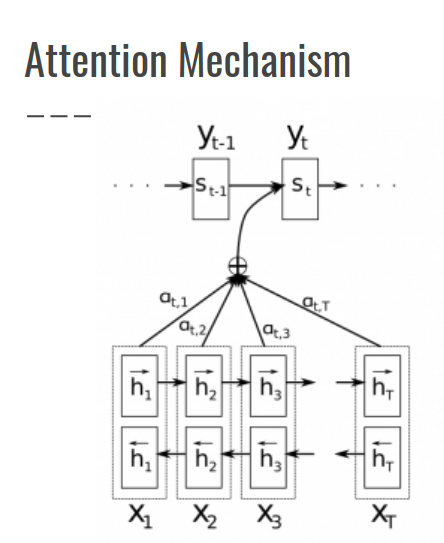
\includegraphics[scale=.3]{attention_mechanism}
\end{center}

\subsection{GRU Variation}
While Bahdanau, et. al.\textsuperscript{[1]} presented the implementation details for the attention
mechanism model, it left open to interpretation a way to apply the model.
In most encoder-decoder architectures, the time cells in the decoder are only built to handle an
input and a previous state, which is often initialized with the encoder’s output.
When we introduced the output of the attention mechanism, which we will refer to as the context,
we could no longer pass it in as the initialization of the state, because the context changes at
every time step of the decoding process.

We decided to treat the context as an additional type of input to keep it separate from the state,
which has a distinct purpose in an RNN.
We propose two context-enhanced GRU architectures that incorporate the context as part of the input
of our time cell.
Cell type A was the simplest alteration we could design.

\begin{center}
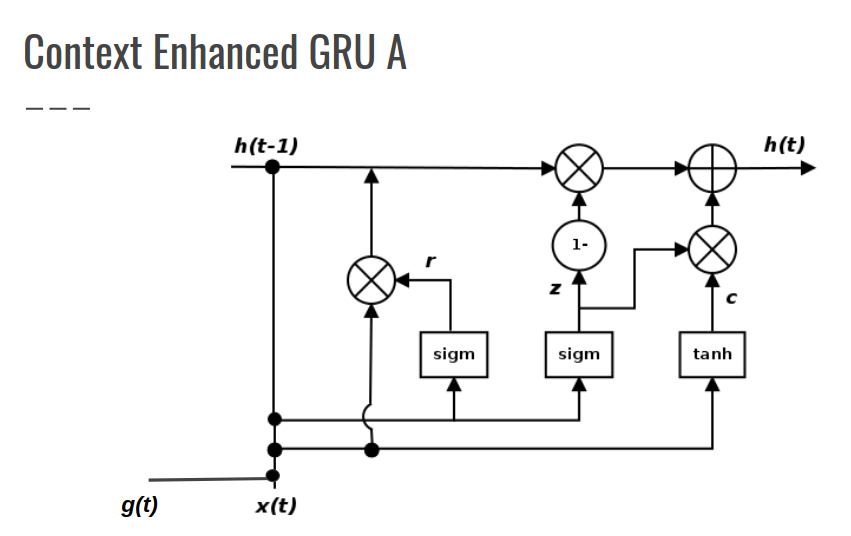
\includegraphics[scale=.2]{context-gru-a}
\end{center}

\noindent It involves simply concatenating the context vector to the input and treating the
concatenation as a new input.
The rest of the cell is identical to a typical GRU.

Cell type B involved passing the state and the context through a fully connected layer and then
through a sigmoid, to create a set of gating coefficients through which to pass the context.

\begin{center}
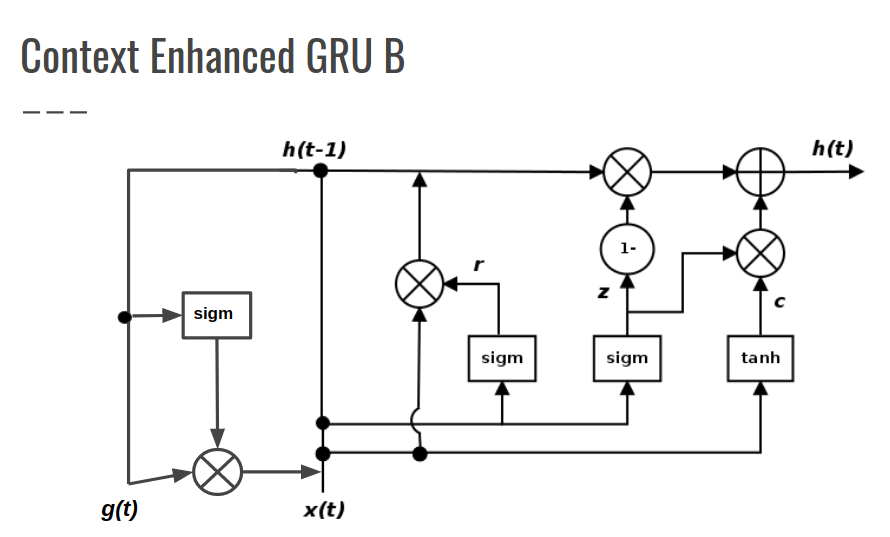
\includegraphics[scale=.2]{context-gru-b}
\end{center}

This enables the model to filter out the irrelevant portions of the context.
The filtered context is then concatenated to the input to create a new input and the remainder of
the cell looks like a typical GRU.

\section{Experiment}

We decided to try our attention mechanism model on an English-to-Spanish NMT task.
We selected a canonical NMT dataset, the European Parliament Proceedings corpus
\textsuperscript{[3]}.
More specifically, we used the subset of this corpus that had aligned English and Spanish sentences.
We knew that our model would have a set output vocabulary size and worried that many of the words
that appeared in our dataset, things such as diverse world leaders, locations, and organizations,
would be too uncommon to be included in our output vocabulary.
Therefore, we used Stanford’s Named Entity Recognition library \textsuperscript{[4]} (NER)
to tag all people, locations, and organizations and replace them with their class name.
We further simplified our translation task by pruning our dataset to preserve only sentences of
length 30 or less composed only of words in the 3000 most common words of the dataset.
We did this for both English and Spanish.

Having simplified our task, we implemented a model that we thought would have sufficient learning
capacity.
Our encoder was a bidirectional RNN where each direction had 2 layers, hidden states of size 256,
and an input size of 300, which was set by the FastText embedding dimension.
It output concatenated hidden states of size 512 as embeddings.
Our decoder was a forward RNN with 2 layers, hidden states of size 512, and an input size of 300.
We used this model size to train 5 different models: a default encoder-decoder model with no
attention mechanism, an attention mechanism based model with cell type A at the first
layer, one with cell type A at every layer, one with cell type B at the first
layer, and one with cell type B at every layer.

We also trained 2 additional models in order to see if increasing model capacity would improve
results.
These were an attention mechanism model with cell type B at the first layer and one with
cell type B at every layer.
However, these models had encoder RNNs with hidden size 512 and a decoder RNN with hidden size
1024.
Moreover, both the encoder and decoder had 3 layers.

For our loss function, since we were trying to predict individual words from a set of 3000, we
thought that cross entropy loss would be appropriate. Since we were trying to do this for an entire
sequence, we averaged cross entropy losses over the entire output sequence and over the batch as
well.

\section{Results}

Our models show a clear trend of learning.
Consider the train and test loss plots, respectively shown below.

\begin{center}
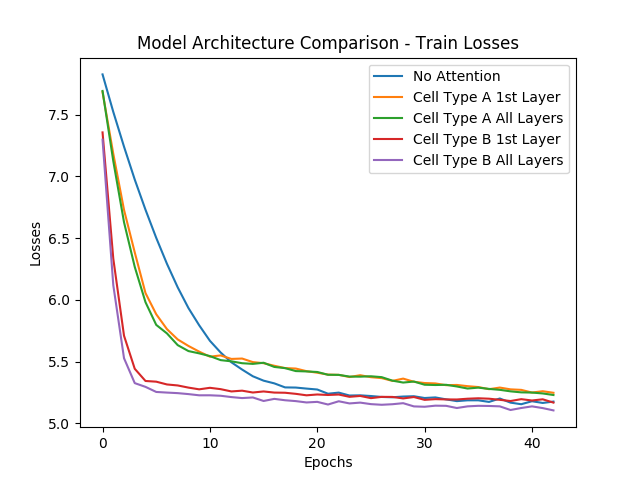
\includegraphics[scale=.4]{model_comparison_losses_train}
\end{center}

\begin{center}
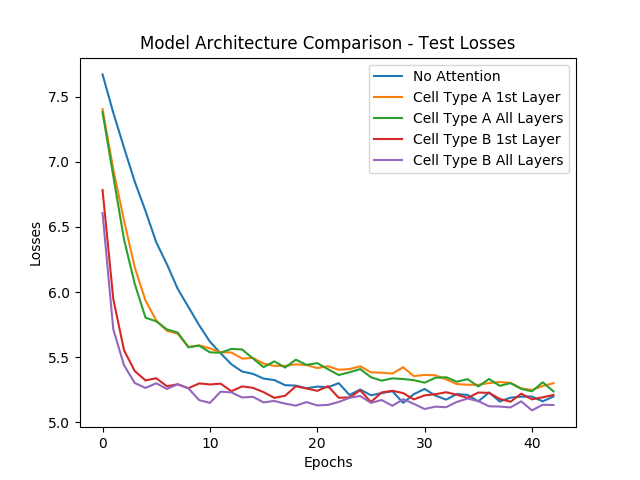
\includegraphics[scale=.4]{model_comparison_losses_test}
\end{center}

\noindent While all models appear to converge to the same minimum, those which use the attention
mechanism begin their convergence more quickly.
The models which use cell type A, plateau sooner, so the model without the attention mechanism
quickly surposes them.
The models with cell type B have better convergence overall.

We also consider a word error rate.
This measurement determines what percentage of the words were incorrectly translated.
Consider the plots below, containing the word error rates for all the models at both train and test
time.

\begin{center}
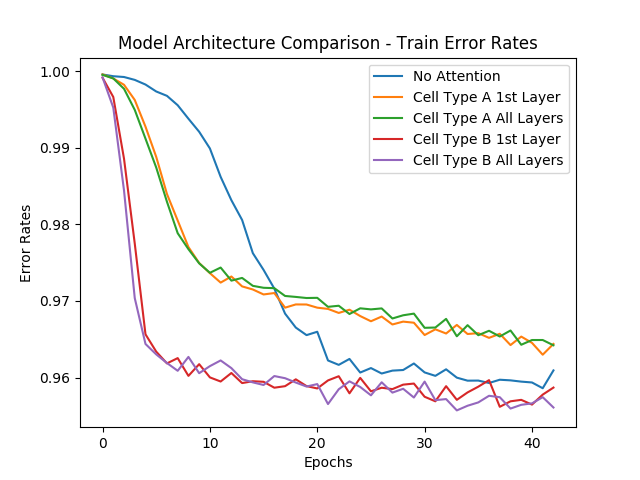
\includegraphics[scale=.4]{model_comparison_error_rates_train}
\end{center}

\begin{center}
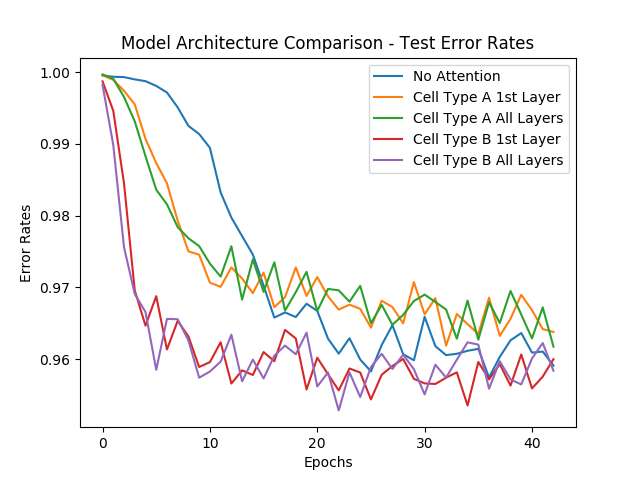
\includegraphics[scale=.4]{model_comparison_error_rates_test}
\end{center}

These word error rates correlate highly with the losses, though with more variance between epochs.

While there is a clear indication of learning some mapping between the English and Spanish text,
word error rates of 96\% are hardly deployable.
We attempted to simplify the learning process from the beginning.
We applied NER to remove the occurances of rare names, places and organizations.
We further reduced the vocab to the most common words.

Attempting to improve our results, we focused on variations on our architectures for the best
architectures, the ones using cell type B.
Since the loss was platteaued quickly, this seemed a reasonable choice.
The loss plots are shown below.

\begin{center}
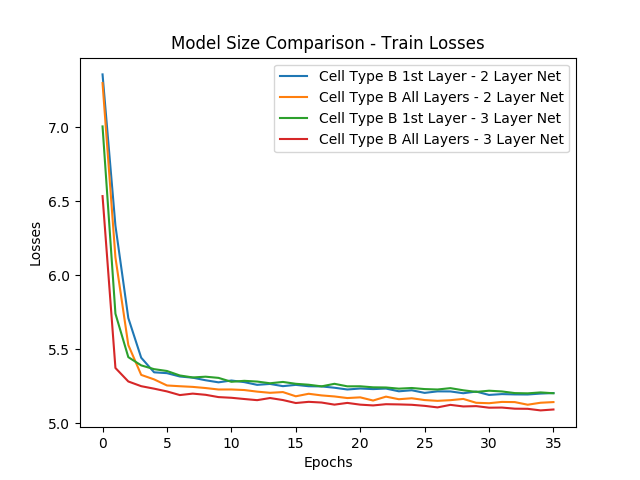
\includegraphics[scale=.4]{size_comparison_losses_train}
\end{center}

\begin{center}
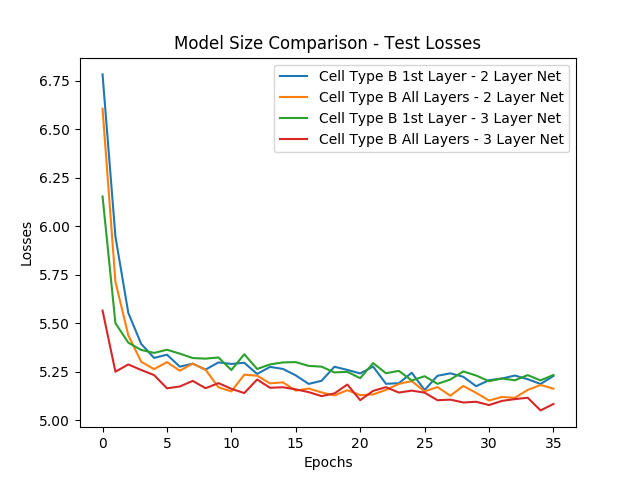
\includegraphics[scale=.4]{size_comparison_losses_test}
\end{center}

\noindent However, changing the hyperparamter settings showed no significant improvement.
There is slight improvement in the capacity of the model when using more layers, as can be expected.

In future iterations, we would consider a couple more variations to lower the word error rate.
It is possible that the models could drop out of their local minima given siginificantly longer
training time.
Furthermore, a differ loss function could ease the task at hand for the models.
Currently, the models are only predicting about one word in 20 correctly, or one word per sentence.
Our loss function does not consider slight variations in word order that could be allowed by the
natural language.

\section{Summary}
Neural machine translation is a difficult task.
A translation dataset requires siginificant natural language processing techniques.
Using an attention mechanism on a traditional RNN allowed us to achieve faster convergence given
the same amount of training data.

\section{Bibliography}
\begin{enumerate}
\item Bahdanau, D., Cho, K., Bengio, Y. "Neural machine translation by jointly learning to align and translate." Proceedings of the International Conference on Learning Representations (ICLR), 2015.

\item K. Cho, B. van Merrienboer, D. Bahdanau, and Y. Bengio. On the properties of neural machine translation: Encoder-decoder approaches. arXiv preprint arXiv:1409.1259, 2014.

\item Europarl: A Parallel Corpus for Statistical Machine Translation, Philipp Koehn, MT Summit 2005.

\item Jenny Rose Finkel, Trond Grenager, and Christopher Manning. 2005. Incorporating Non-local Information into Information Extraction Systems by Gibbs Sampling. Proceedings of the 43nd Annual Meeting of the Association for Computational Linguistics (ACL 2005), pp. 363-370. http://nlp.stanford.edu/~manning/papers/gibbscrf3.pdf
\end{enumerate}

\end{multicols}
\end{document}
